%-------------------------------------------------------------------------------
\section{Mathematical / physical description}\label{sec:method}
%-------------------------------------------------------------------------------
In the following, we describe the SKYCORR sky correction procedure in more
detail (also see Section~\ref{sec:algorithm}). First, we discuss how emission
lines are identified in the input science and sky spectra
(Section~\ref{sec:linesearch}). This procedure also derives the typical line
FWHM (Section~\ref{sec:linesearch}). Next, the subtraction of the remaining
continua from the identified line spectra is described
(Section~\ref{sec:contsub}). Then, the airglow model is discussed
(Section~\ref{sec:airglow}). It is an essential input for scaling the
reference sky line spectrum to fit the science line spectrum
(Section~\ref{sec:linefit}). The fitting procedure also allows adapting the
wavelength grids (Section~\ref{sec:wavegrid}). The final step of the sky
correction procedure is the sky subtraction itself. This operation is just the
subtraction of the best-fit sky line spectrum and the unscaled sky continuum
spectrum from the input science spectrum (see also
Section~\ref{sec:algorithm}).

%-------------------------------------------------------------------------------
\subsection{Line finder}\label{sec:linesearch}
%-------------------------------------------------------------------------------
The sky correction procedure focuses on fitting the airglow emission lines in
an input science spectrum by scaling a reference sky line spectrum. Hence,
object and sky continua have to be subtracted in advance. This requires
identification of line and continuum pixels in the input spectra. Spectral
lines are identified by an approach that uses the first derivative of the
spectrum. Thus, line pixels can be recognised by their large flux gradients.
Emission line peaks can be identified by a change from positive to negative
values of the first derivative.

\begin{figure}
\centering
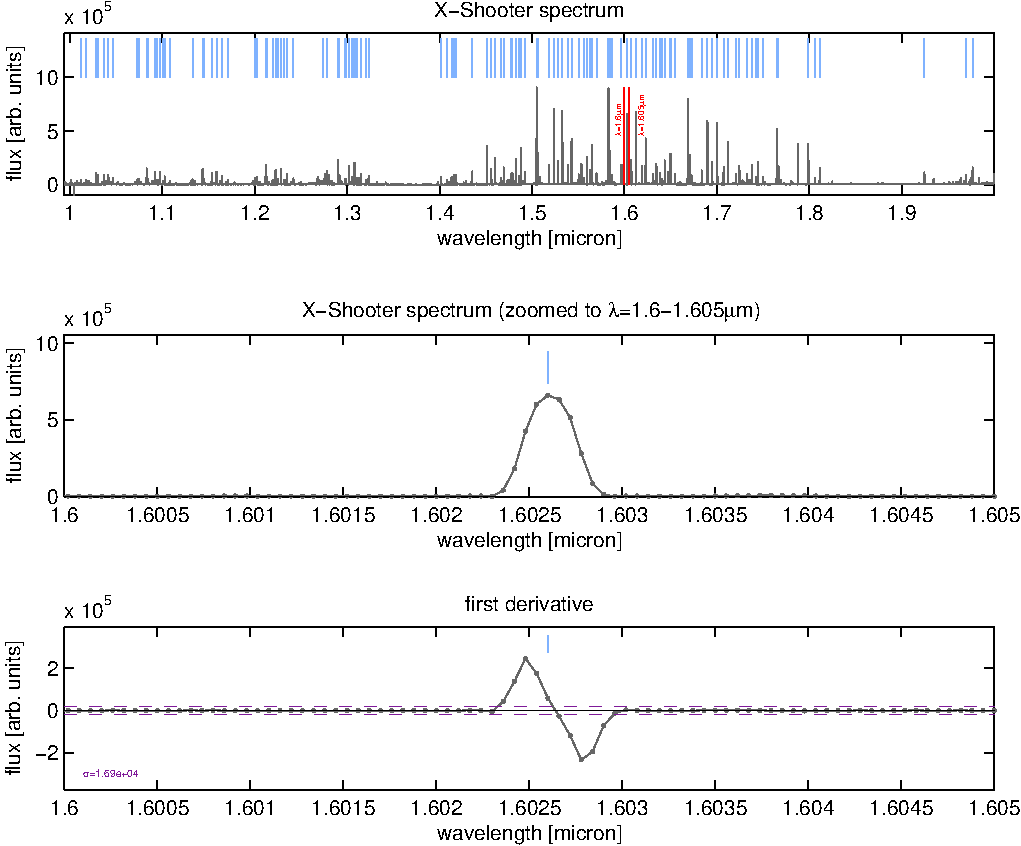
\includegraphics[width=17cm,clip=true]
{figures/X-Shooter_spec_deriv_1_6-1_605.pdf}
\caption[]{X-Shooter sky spectrum {\tt sky\_xshoo\_28}. The upper panel shows
the entire wavelength range $\lambda=1.0...2.0\,\mu$m with the zoom range
$\lambda=1.6...1.605\,\mu$m (red lines) shown in the middle panel containing a
prominent single emission line. In the lower panel the first derivative of this
line is given, which shows a significant change in the values. Such changes
are used as signature to identify emission lines (marked by the light blue
vertical lines in the panels).}
\label{fig:xshoo1}
\end{figure}

\begin{figure}
\centering
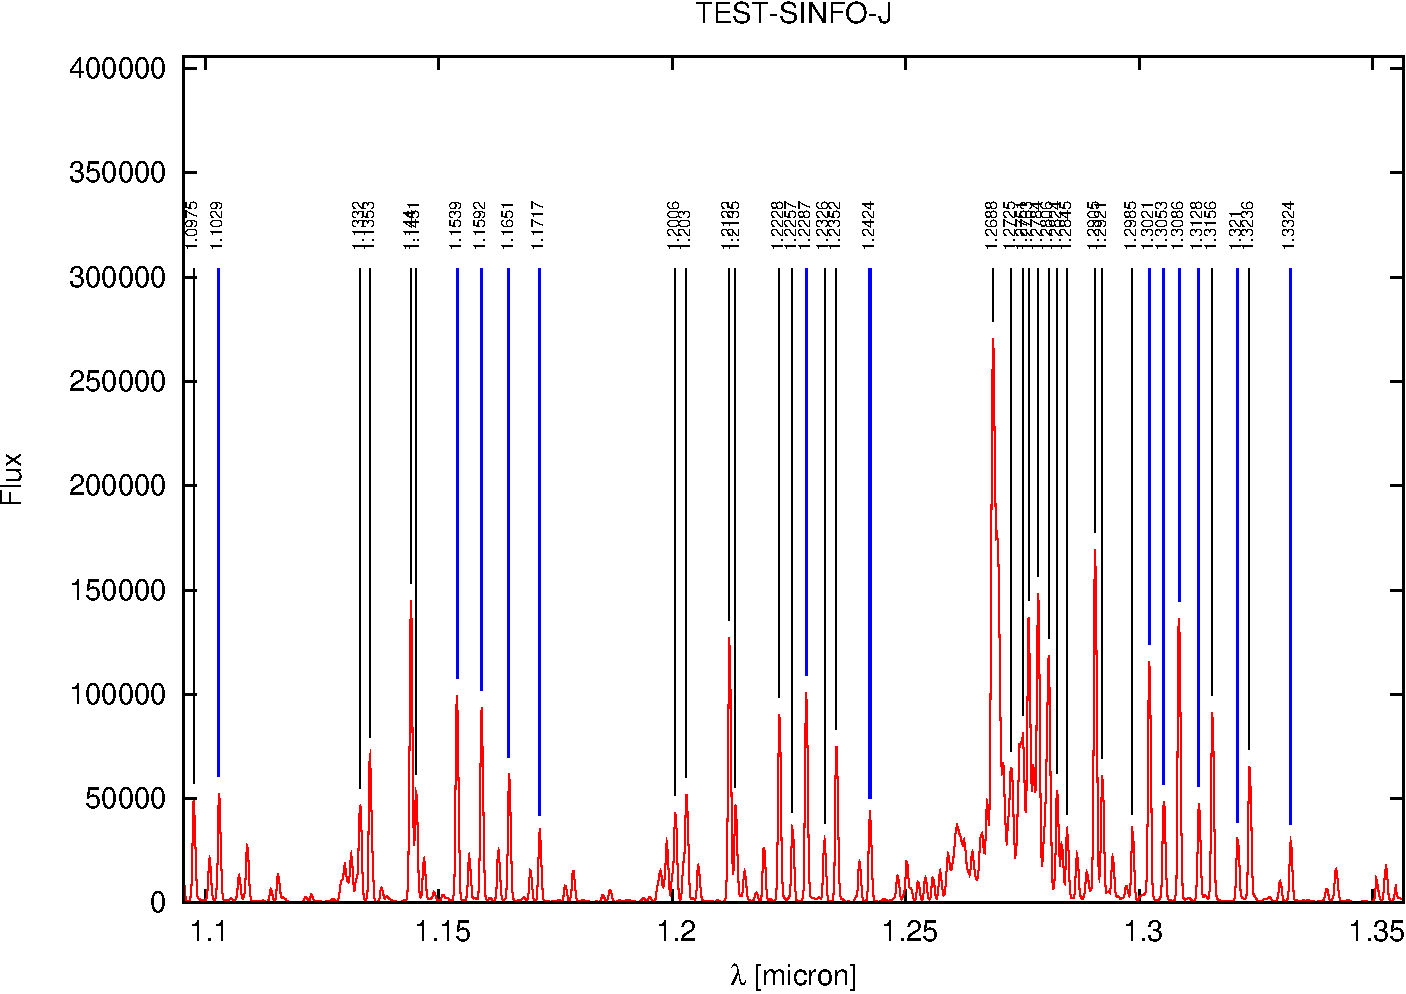
\includegraphics[width=9.5cm,clip=true]
{figures/TEST-SINFO-J_with_lines.pdf}
\caption[]{SINFONI $J$-band sky spectrum with detected emission lines
(blue = isolated lines used for the FWHM estimate).}
\label{fig:sinfoj1}
\end{figure}

\begin{figure}
\centering
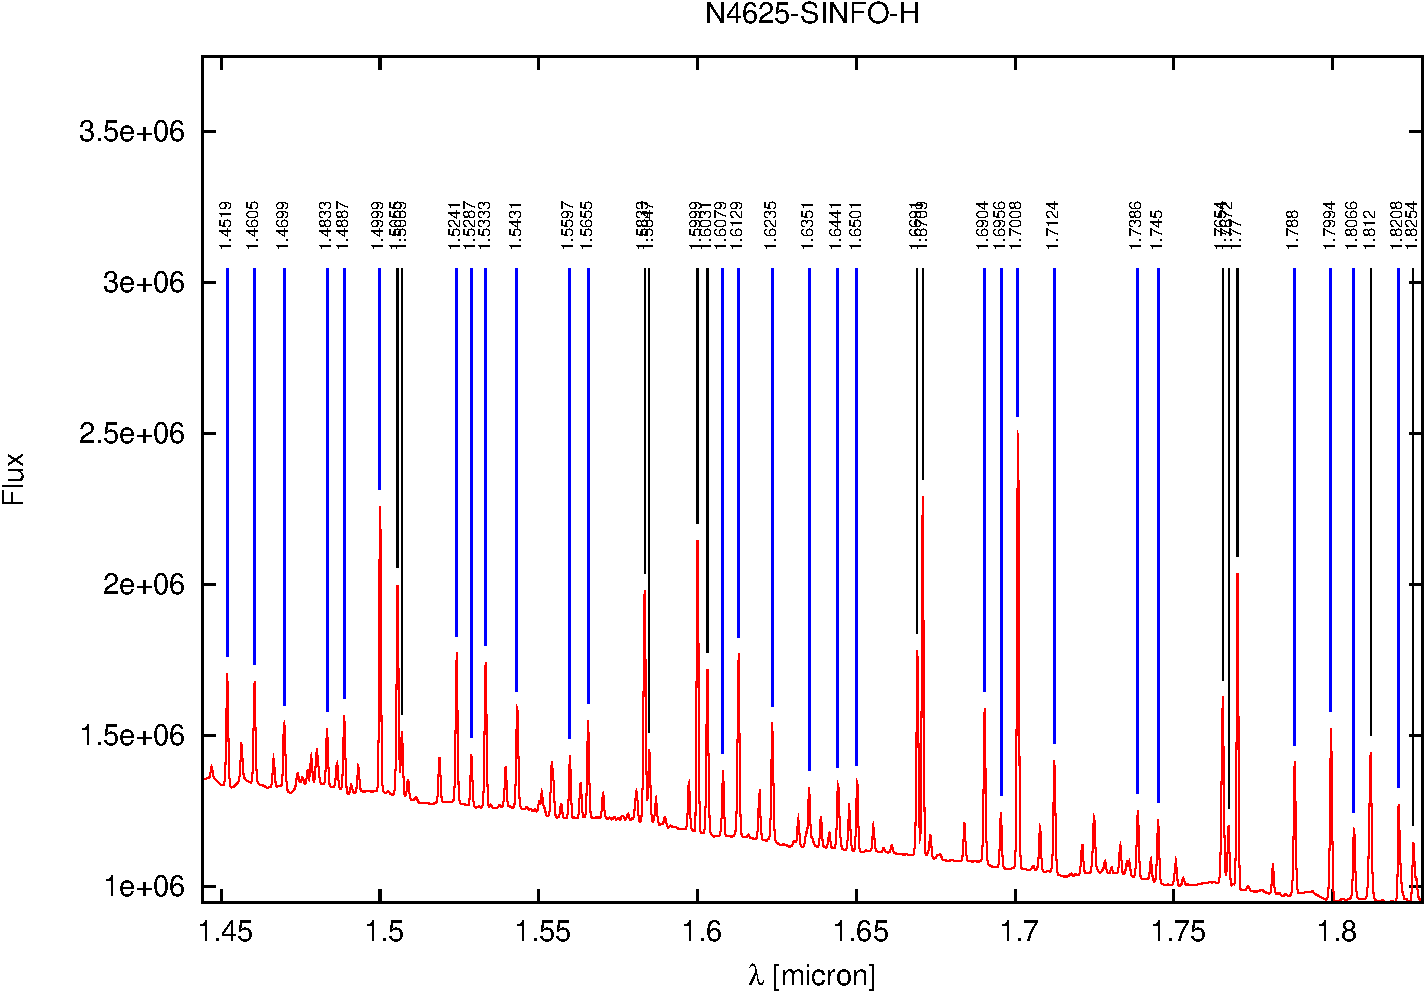
\includegraphics[width=9.5cm,clip=true]
{figures/N4625-SINFO-H_with_lines.pdf}
\caption[]{SINFONI $H$-band sky spectrum + arbitrarily scaled NGC\,4625
spectrum at $z = 0.5$ + 5 artificial emission lines of equal intensity with
detected emission lines (blue = isolated lines used for the FWHM estimate).}
\label{fig:sinfoh1}
\end{figure}

Figure~\ref{fig:xshoo1} shows the X-Shooter spectrum {\tt sky\_xshoo\_28} (see
Section~\ref{sec:evaluation}) in the upper panel. A zoom-in to the wavelength
range $\lambda=1.6...1.605\,\mu$m isolates a prominent single emission line
(middle panel). The first derivative of the same spectral range (lower panel)
reveals a significant change from positive to negative values allowing
detection of emission lines. Single emission lines are identified by this
particular signature. Note that only changes $\geq1\sigma$ above the noise
level are taken into account to avoid spurious detections from noise or broad
lines caused by blending.

Line identification via the first derivative allows robust characterisation of
lines also in case of strong (pseudo)\-continuum variations. This is necessary
as isolated lines are required for estimating their FWHM.
Figures~\ref{fig:sinfoj1} and \ref{fig:sinfoh1} show a SINFONI $J$-band and
$H$-band spectrum, respectively. In the latter a simulated object
spectrum was added to the sky emission (see Section~\ref{sec:evaluation} for
more information). The distinct emission peak at $\lambda\sim1.25....1.3\,\mu$m
in the $J$-band is a pseudocontinuum caused by many unresolved O$_2$ sky lines,
whereas in the $H$-band observation a real continuum is visible. In both cases,
individual emission lines could be identified.

All detected lines are assembled in a line list, which is refined by an
iterative method depending on the estimation of the sky line FWHM (see
Section~\ref{sec:FWHM}). This procedure requires identification of strong,
isolated lines. Therefore, the line finder checks the previously identified
line peaks, applying criteria characterising isolated lines. For a line to be
marked as isolated, it has to be sufficiently separated from other lines and
its peak has to have a symmetric shape. The first criterion can be influenced
by the user. The parameter file includes the unitless scaling parameter {\sc
min\_line\_dist} that is internally multiplied by the line FWHM in pixels.
Also, this parameter is included in the driver file (see
Section~\ref{sec:params}). Since the FWHM is optimised in an iterative
procedure (see Section~\ref{sec:FWHM}), the given value in the file is only
used as first guess.

For strong and well separated lines, the described line finding method is very
robust. However, for low resolution spectra with many blended lines a major
fraction of lines may be missed. Therefore, the line list of the airglow model
is being used (see Section~\ref{sec:airglow}) to find previously unidentified
lines that have fluxes above the median flux of the lines identified by the
derivative approach times the {\sc fluxlim} parameter of the parameter file. By
default, {\sc fluxlim} is set to -1, which indicates an iterative approach
starting with 0.005 and doubling the previous value in subsequent iterations.
If the higher limit does not spare sufficient continuum pixels for the
continuum interpolation (see Section~\ref{sec:contsub}), \ie\ at least 20\% of
all pixels distributed over more than 90\% of the wavelength range, the
procedure is stopped and 0.005 is eventually selected, otherwise the threshold
value is doubled (\ie\ 0.02 is taken). This process is repeated as long as a
sufficient number of continuum pixels are left over or a value of 0.08 is
reached. The number of pixels characterised as line pixels for each line
included from the line list depends on the given line FWHM (see above and
Section~\ref{sec:FWHM}). The combination of line pixels identified by both
methods gives a good estimate of the spectral ranges covered by significant
airglow lines (see Figure~\ref{fig:lineflags}).

\begin{figure}
\centering
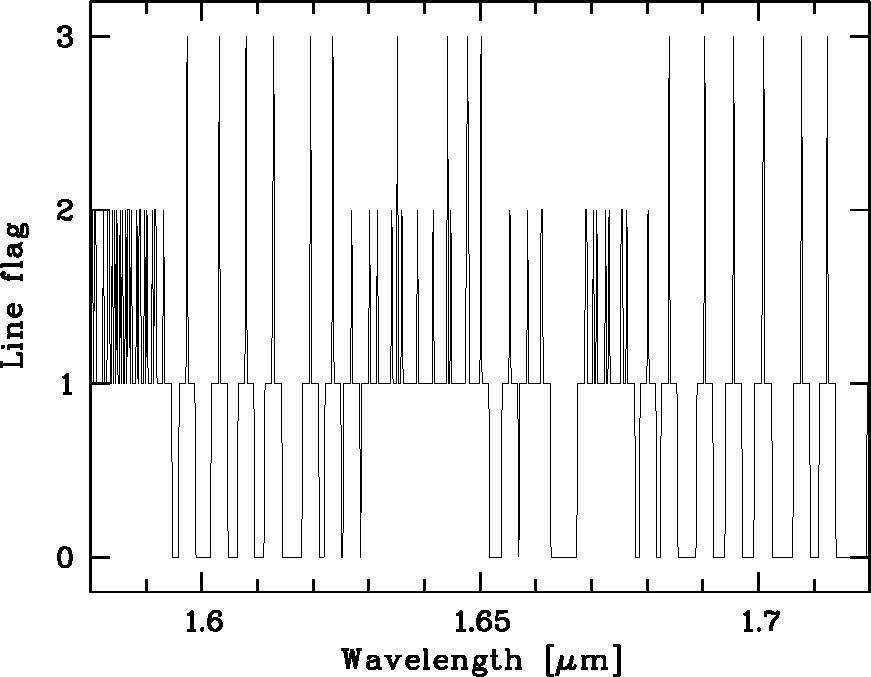
\includegraphics[width=12cm,clip=true]{figures/scd_illlineflags.pdf}
\caption[]{Line flags identified in a part of a SINFONI $H$-band spectrum. The
meaning of the flags is as follows: 0 = continuum, 1 = line pixel,
2 = line peak, 3 = isolated line peak.}
\label{fig:lineflags}
\end{figure}

%-------------------------------------------------------------------------------
\subsection{Line FWHM estimator}\label{sec:FWHM}
%-------------------------------------------------------------------------------
For calculating the airglow model (see Section~\ref{sec:airglow}), it is
required to convert total line fluxes as provided by the input line list into
fluxes per wavelength interval. Consequently, it is necessary to know the
typical FWHM of the airglow lines, which is the only line shape parameter
assuming a Gaussian line profile. The line finder described in the previous
Section~\ref{sec:linesearch} searches for isolated lines that are suitable for
deriving a FWHM. After the subtraction of the continuum (see
Section~\ref{sec:contsub}), the FWHM estimation can be performed by fitting a
Gaussian to the line pixels belonging to each isolated line. For the fitting
procedure, the C version of the least-squares fitting library MPFIT by
C.~Markwardt~\cite{CMPFIT} based on the FORTRAN fitting routine MINPACK-1 by
Mor\'e et al.~\cite{MOR80} is used (see also Section~\ref{sec:linefit}).
The FWHM measurements of all isolated lines are averaged to obtain the typical
FWHM of the input spectrum. In order to avoid blended lines contributing to
the resulting mean, a $\sigma$-clipping approach is applied to skip
suspiciuosly high FWHM. The method is based on computing the median absolute
difference between the data points and their median and the subsequent
application of Huber's method for an iterative clipping of outliers
\cite{huber} and the derivation of reliable mean and standard deviation from
the unclipped values. If less than five isolated lines remain after clipping,
the median FWHM is taken.

The fact that the estimated value of the FWHM affects the search for isolated
lines (see Section~\ref{sec:linesearch}), which are required for the FWHM
estimation, necessitates an iterative approach in which line finder, continuum
subtractor, and FWHM estimator are called several times in turn in order to
obtain a stable and trustworthy FWHM. This iterative procedure is terminated if
convergence is reached for the mean FWHM. The convergence criterion is
provided by the parameter {\sc ltol} (see Section~\ref{sec:params}).

For instruments like X-Shooter, whose spectra show a roughly linear increase of
the FWHM with wavelength, this can be considered by the setting the parameter
{\sc varfwhm} to 1. In this case, the FWHM estimates of the individual lines
are converted to correspond to the FWHM, which would be measured at the
central wavelength of the full spectrum, assuming a linear change of the
FWHM with wavelength. The converted FWHM are then used to calculate the mean
FWHM as discussed above. The linear change of the FWHM is also considered for
the separation of lines and continuum (see Section~\ref{sec:linesearch}) and
the calculation of the pixel contributions of the different line groups
(see Section~\ref{sec:linefit}).

%-------------------------------------------------------------------------------
\subsection{Continuum subtraction}\label{sec:contsub}
%-------------------------------------------------------------------------------
\begin{figure}
\centering
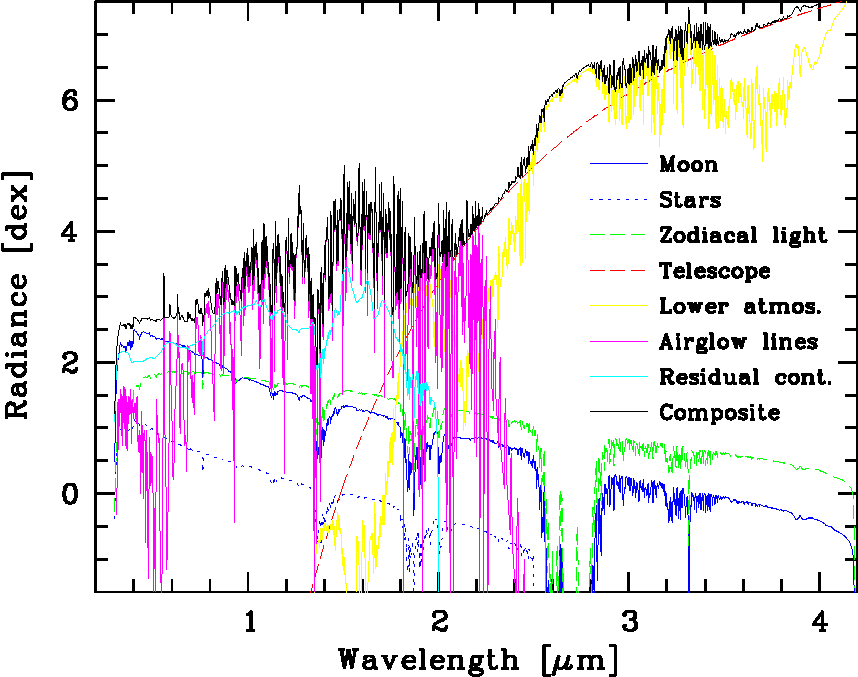
\includegraphics[width=12cm,clip=true]{figures/smd2_logcomp.pdf}
\caption[]{Components of the SM-01 sky model for wavelengths between $0.3$ and
6\,$\mu$m in logarithmic flux units. The example with Moon above the horizon
shows the scattered moonlight, scattered starlight, zodiacal light, thermal
emission by telescope and instrument, molecular emission of the lower
atmosphere, airglow emission lines of the upper atmosphere, and
airglow/residual continuum.}
\label{fig:logcomp}
\end{figure}

The adaptation of the reference sky line spectrum to the airglow lines in the
input science spectrum by multiplying factors to physically motivated line
groups (see Section~\ref{sec:airglow}) requires that any kind of continuum is
subtracted before this procedure. In particular, the object continuum can cause
problems, since it is not present in the reference sky spectrum. However, sky
spectra also show continuum emission. The main components are scattered
moonlight, scattered starlight, zodiacal light, thermal emission from the lower
atmosphere by greenhouse gases and the telescope itself, and airglow continuum
emission, which is related most probably to chemiluminescent reactions in the
upper atmosphere involving nitric oxide (see Section~\ref{sec:airglow}, Noll et
al.~\cite{NOL12}, and Khomich et al.~\cite{KHO08} and references therein). As
Figure~\ref{fig:logcomp} indicates, the main continuum component is the
airglow/residual continuum\footnote{Note that this component is very difficult
to determine. Its measured intensity strongly depends on the accuracy of the
other components, the quality of the flux calibration, and possible
instrumental continua. For this reason, it should also been seen as residual
continuum.}, which dominates shortwards of the thermal regime with the
exception of the UV and optical if the Moon is up. The variable airglow
continuum (see Figure~\ref{fig:illfeatvar}) cannot be corrected by a fitting
procedure like for the airglow lines (see Section~\ref{sec:airglow}), since
object and sky continuum cannot be separated in the science spectrum (cf.
Section~\ref{sec:davies}). Therefore, it has to be assumed that the sky
continuum in the science spectrum does not differ much from the one in the
reference sky spectrum. If this requirement is fulfilled, a simple subtraction
of the continua in both input spectra of the sky correction procedure should
provide results with good quality.

SKYCORR obtains the continua in the input science and sky spectra using line
identification flags (see Figure~\ref{fig:lineflags}) set in the course of the
line search described in Section~\ref{sec:linesearch}. All pixels not flagged
as line pixels are connected by linear interpolation. Thorough identification
of continuum pixels guaranteed, this is the most efficient approach even in the
case of line blends covering wide wavelength ranges.

%-------------------------------------------------------------------------------
\subsection{Airglow model}\label{sec:airglow}
%-------------------------------------------------------------------------------
\begin{figure}
\centering
\includegraphics[width=10cm,clip=true]{figures/varclasses.eps}
\caption[]{Variability classes for sky emission lines. The following groups are
defined: green O\,I, Na\,I\,D, red O\,I, OH, and O$_2$. The weak lines (green
curves) are scaled by a factor of 30 for Na\,I\,D, red O\,I, and O$_2$, and a
factor of 10 for OH.}
\label{fig:varclasses}
\end{figure}

\begin{figure}
\centering
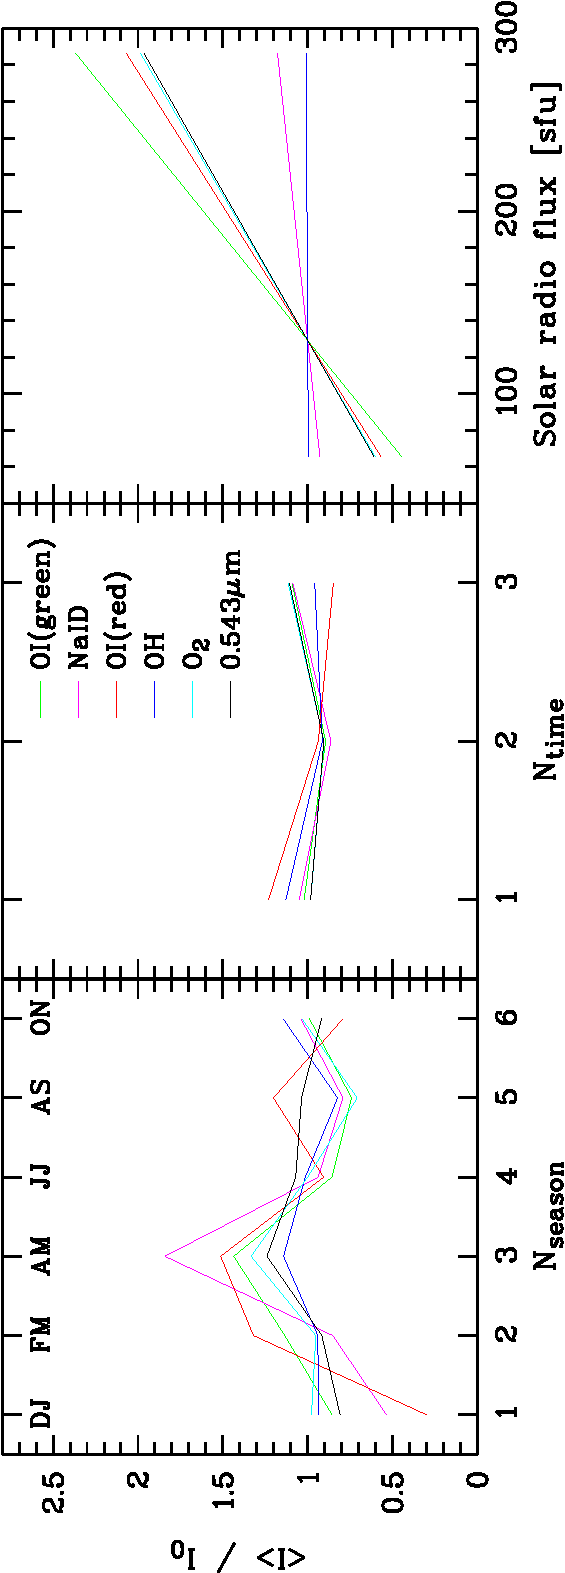
\includegraphics[height=\textwidth,angle=-90,clip=true]
{figures/scd_illfeatvar.pdf}
\caption[]{Variability correction for the five sky line classes and the
airglow continuum of the sky model. The variability is shown as a function of
the bimonthly period (1 = Dec/Jan, ..., 6 = Oct/Nov), time bin (third of the
night), and the solar activity measured by the solar radio flux
(sfu~$= 0.01$\,MJy).}
\label{fig:illfeatvar}
\end{figure}

\begin{table}
\caption[]{Description of A groups in the input line list}
\label{tab:Agroups}
\centering
\footnotesize
\vspace{5pt}
\begin{tabular}{c c c l}
\hline\hline
\noalign{\smallskip}
ID & $N_\mathrm{lin}$ & Wavelength range [\mum] & Description \\
\noalign{\smallskip}
\hline
\noalign{\smallskip}
 1 &  61 & 0.314 - 0.872 & green O\,I at 0.5577\,$\mu$m + unidentified lines \\
 2 &   3 & 0.589 - 0.770 & Na\,I\,D + other lines from alkali metals \\
 3 &  23 & 0.389 - 0.845 & red O\,I at 0.6300\,$\mu$m + other thermospheric
                           lines \\
 4 &   1 & 0.467 - 0.467 & OH(7-0) \\
 5 &   8 & 0.491 - 0.495 & OH(8-1) \\
 6 &  22 & 0.519 - 0.536 & OH(9-2) \\
 7 &  12 & 0.526 - 0.535 & OH(6-0) \\
 8 &  23 & 0.554 - 0.570 & OH(7-1) \\
 9 &  41 & 0.587 - 0.634 & OH(8-2) \\
10 &  49 & 0.624 - 0.655 & OH(9-3) \\
11 &   2 & 0.672 - 0.674 & OH(10-4) \\
12 &  27 & 0.614 - 0.695 & OH(5-0) \\
13 &  83 & 0.647 - 0.754 & OH(6-1) \\
14 & 113 & 0.681 - 0.782 & OH(7-2) \\
15 & 111 & 0.720 - 0.815 & OH(8-3) \\
16 &  72 & 0.768 - 0.822 & OH(9-4) \\
17 &   7 & 0.827 - 0.839 & OH(10-5) \\
18 &  85 & 0.745 - 0.910 & OH(4-0) \\
19 & 113 & 0.781 - 0.914 & OH(5-1) \\
20 & 111 & 0.826 - 0.916 & OH(6-2) \\
21 & 110 & 0.873 - 0.937 & OH(7-3) \\
22 & 116 & 0.931 - 1.007 & OH(8-4) \\
23 & 120 & 0.994 - 1.081 & OH(9-5) \\
24 & 100 & 0.965 - 1.043 & OH(3-0) \\
25 & 110 & 1.015 - 1.098 & OH(4-1) \\
26 & 112 & 1.069 - 1.168 & OH(5-2) \\
27 & 118 & 1.129 - 1.236 & OH(6-3) \\
28 & 120 & 1.197 - 1.314 & OH(7-4) \\
29 & 124 & 1.275 - 1.420 & OH(8-5) \\
30 & 128 & 1.366 - 1.531 & OH(9-6) \\
31 & 112 & 1.392 - 1.558 & OH(2-0) \\
32 & 118 & 1.461 - 1.654 & OH(3-1) \\
33 & 122 & 1.537 - 1.743 & OH(4-2) \\
34 & 122 & 1.622 - 1.842 & OH(5-3) \\
35 & 124 & 1.717 - 1.978 & OH(6-4) \\
36 & 126 & 1.825 - 2.110 & OH(7-5) \\
37 & 130 & 1.951 - 2.265 & OH(8-6) \\
38 & 130 & 2.101 - 2.454 & OH(9-7) \\
39 & 450 & 0.314 - 0.532 & O$_2$(A-X) (Herzberg I) \\
40 &   5 & 0.324 - 0.410 & O$_2$(c-X) (Herzberg II) \\
41 & 396 & 0.326 - 0.550 & O$_2$(A'-a) (Chamberlain) \\
42 &  65 & 0.382 - 0.509 & O$_2$(c-b) \\
43 & 208 & 0.656 - 0.806 & O$_2$(b-X) (v' > v'') \\
44 & 194 & 0.761 - 0.816 & O$_2$(b-X) (v' = v'') \\
45 & 103 & 0.861 - 0.922 & O$_2$(b-X) (v' < v''; atmospheric 0-1 band
                           inclusive) \\
46 & 161 & 1.240 - 1.305 & O$_2$(a-X)(0-0) (IR atmospheric system) \\
47 &  73 & 1.555 - 1.598 & O$_2$(a-X)(0-1) (IR atmospheric system) \\
\noalign{\smallskip}
\hline
\end{tabular}
\end{table}

\begin{table}
\caption[]{Description of B groups in the input line list}
\label{tab:Bgroups}
\centering
\footnotesize
\vspace{5pt}
\begin{tabular}{c c l l}
\hline\hline
\noalign{\smallskip}
ID & Molecule & Upper state(s) & Remarks$^\mathrm{a}$ \\
\noalign{\smallskip}
\hline
\noalign{\smallskip}
 1 & OH & $X^2\Pi_{1/2}$, $J' = 1/2$  & Q2(0.5), P2(1.5) \\
 2 & OH & $X^2\Pi_{3/2}$, $J' = 3/2$  & Q1(1.5), P1(2.5) \\
 3 & OH & $X^2\Pi_{1/2}$, $J' = 3/2$  & R2(0.5), Q2(1.5), P2(2.5) \\
 4 & OH & $X^2\Pi_{3/2}$, $J' = 5/2$  & R1(1.5), Q1(2.5), P1(3.5) \\
 5 & OH & $X^2\Pi_{1/2}$, $J' = 5/2$  & R2(1.5), Q2(2.5), P2(3.5) \\
 6 & OH & $X^2\Pi_{3/2}$, $J' = 7/2$  & R1(2.5), Q1(3.5), P1(4.5) \\
 7 & OH & $X^2\Pi_{1/2}$, $J' = 7/2$  & R2(2.5), Q2(3.5), P2(4.5) \\
 8 & OH & $X^2\Pi_{3/2}$, $J' = 9/2$  & R1(3.5), Q1(4.5), P1(5.5) \\
 9 & OH & $X^2\Pi_{1/2}$, $J' = 9/2$  & R2(3.5), Q2(4.5), P2(5.5) \\
10 & OH & $X^2\Pi_{3/2}$, $J' = 11/2$ & R1(4.5), Q1(5.5), P1(6.5) \\
11 & O$_2$ & $b^1\Sigma^+_g$, $J' = 0, 2, 4$ & \\
12 & O$_2$ & $b^1\Sigma^+_g$, $J' = 6, 8$ & \\
13 & O$_2$ & $b^1\Sigma^+_g$, $J' = 10, 12$ & \\
14 & O$_2$ & $b^1\Sigma^+_g$, $J' = 14, 16$ & \\
15 & O$_2$ & $a^1\Delta_g$, $J' = 2, 4$ & $v'' = 0$ \\
16 & O$_2$ & $a^1\Delta_g$, $J' = 6, 8$ & $v'' = 0$ \\
17 & O$_2$ & $a^1\Delta_g$, $J' = 10, 12$ & $v'' = 0$ \\
18 & O$_2$ & $a^1\Delta_g$, $J' = 14, 16$ & $v'' = 0$ \\
19 & O$_2$ & $a^1\Delta_g$, $J' = 18, 20$ & $v'' = 0$ \\
20 & O$_2$ & $a^1\Delta_g$, $J' = 20, 22$ & $v'' = 0$ \\
21 & O$_2$ & $a^1\Delta_g$, $J' = 2, 4$ & $v'' \ne 0$ \\
22 & O$_2$ & $a^1\Delta_g$, $J' = 6, 8$ & $v'' \ne 0$ \\
23 & O$_2$ & $a^1\Delta_g$, $J' = 10, 12$ & $v'' \ne 0$ \\
24 & O$_2$ & $a^1\Delta_g$, $J' = 14, 16$ & $v'' \ne 0$ \\
\noalign{\smallskip}
\hline
\end{tabular}
\footnotesize
\begin{list}{}{}
\item[$^\mathrm{a}$] OH rotational transitions or lower vibrational level for
O$_2$(a-X) transitions
\end{list}
\end{table}

\begin{figure}
\centering
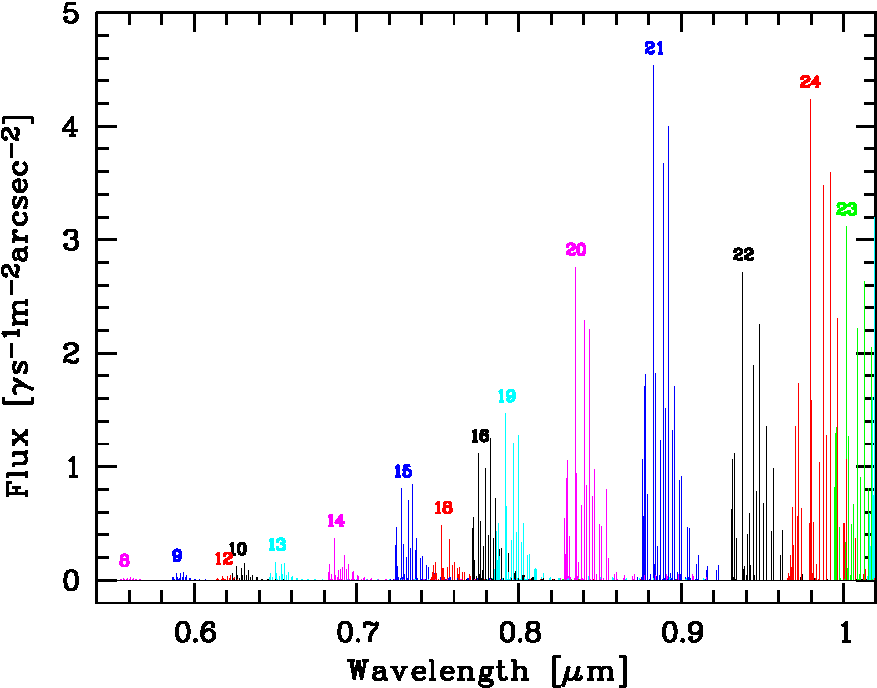
\includegraphics[width=10cm,clip=true]
{figures/scd_plotohbands_opt.pdf}
\caption[]{A group identifications of OH bands (cf. Table~\ref{tab:Agroups}) in
the wavelength range between 0.54 and 1.02\,\mum{} that have Q1(1.5) lines
(see Table~\ref{tab:Bgroups} and Figure~\ref{fig:ohband}) stronger than
0.01\,$\gamma\,{\rm s}^{-1}\,{\rm m}^{-2}\,{\rm arcsec}^{-2}$. The wavelengths and
zenithal mean fluxes (considering absorption in the lower atmosphere) tabulated
in the input line list are plotted. Note that the bands with numbers up to 21
appear twice as strong as the bands at longer wavelengths, since the
corresponding lines were taken from the Hanuschik \cite{HAN03} atlas, where OH
doublets are often unresolved and are listed as one line only.}
\label{fig:ohbands_opt}
\end{figure}

\begin{figure}
\centering
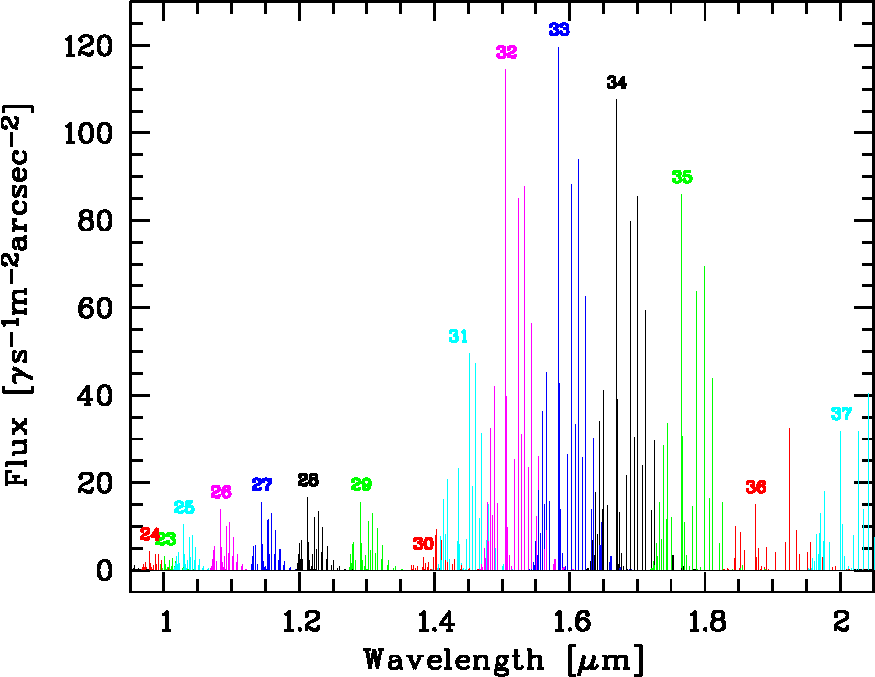
\includegraphics[width=10cm,clip=true]
{figures/scd_plotohbands_ir.pdf}
\caption[]{A group identifications of the OH bands (cf.
Table~\ref{tab:Agroups}) in the wavelength range between 0.95 and 2.05\,\mum{}.
The wavelengths and zenithal mean fluxes tabulated in the input line list are
plotted.}
\label{fig:ohbands_ir}
\end{figure}

\begin{figure}
\centering
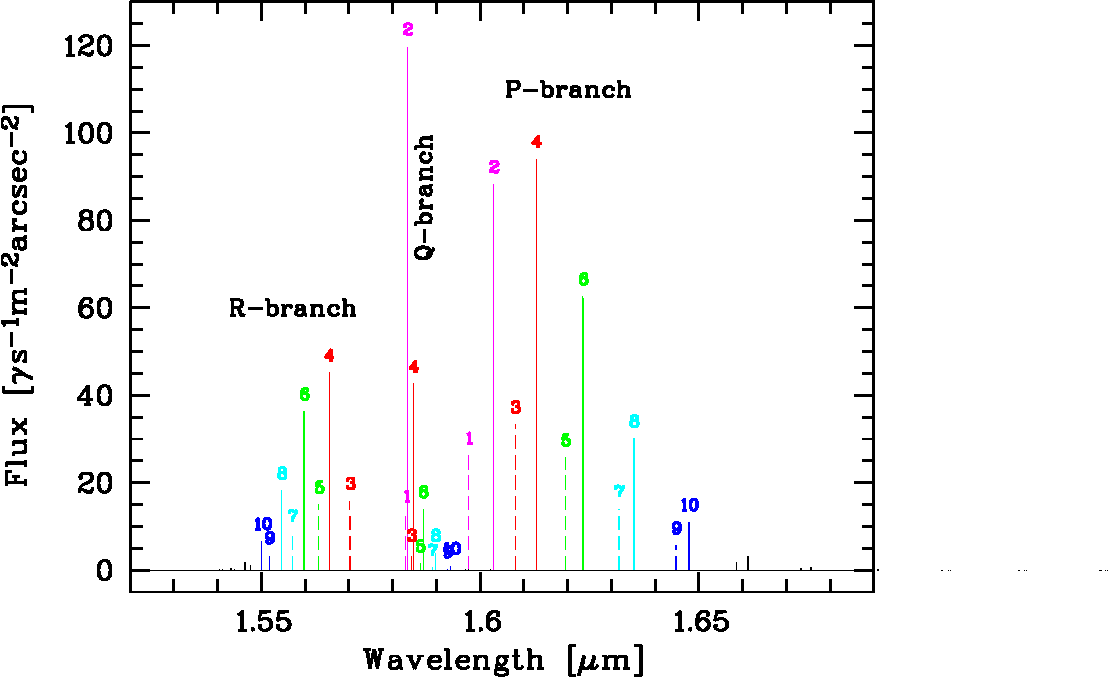
\includegraphics[width=10cm,clip=true]
{figures/scd_plotohband.pdf}
\caption[]{B group identifications of the transitions of an OH band with the
same rotational upper state (cf. Table~\ref{tab:Bgroups}). The tabulated
wavelengths and zenithal mean fluxes of the lines of the OH(6-4) band are shown
as example. Dashed and solid lines indicate transitions of the $X^2\Pi_{1/2}$ and
$X^2\Pi_{3/2}$ state, respectively. The figure also indicates the R-, Q-, and
P-branches that correspond to transitions with a change of the total angular
momentum by -1, 0, and 1, respectively.}
\label{fig:ohband}
\end{figure}

\begin{figure}
\centering
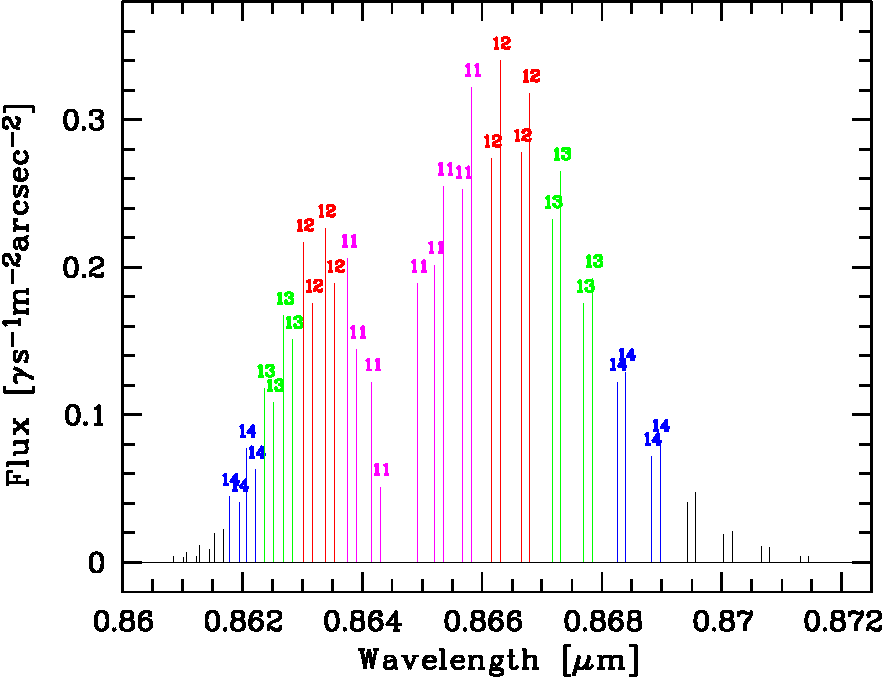
\includegraphics[width=10cm,clip=true]
{figures/scd_ploto2b01band.pdf}
\caption[]{B group identifications of the transitions of the band
O$_2$(b-X)(0-1) with a similar rotational upper state (cf.
Table~\ref{tab:Bgroups}). The tabulated wavelengths and zenithal mean fluxes of
the lines of the 4 different branches (2 R- and 2 P-branches) are shown (cf.
Figure~\ref{fig:ohband}).}
\label{fig:o2b01band}
\end{figure}

\begin{figure}
\centering
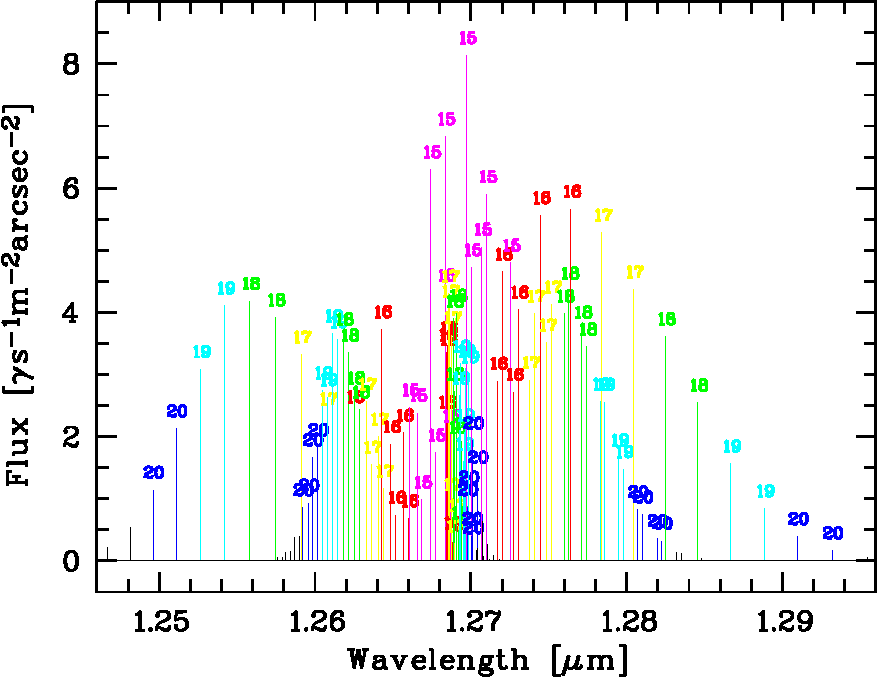
\includegraphics[width=10cm,clip=true]
{figures/scd_ploto2a00band.pdf}
\caption[]{B group identifications of the transitions of the band
O$_2$(a-X)(0-0) with a similar rotational upper state (cf.
Table~\ref{tab:Bgroups}). The tabulated wavelengths and zenithal mean fluxes of
the lines of the 9 different branches (3 R-, 3 Q-, and 3 P-branches) are shown
(cf. Figure~\ref{fig:ohband}). The band is strongly affected by self
absorption in the lower atmosphere.}
\label{fig:o2a00band}
\end{figure}

\begin{figure}
\centering
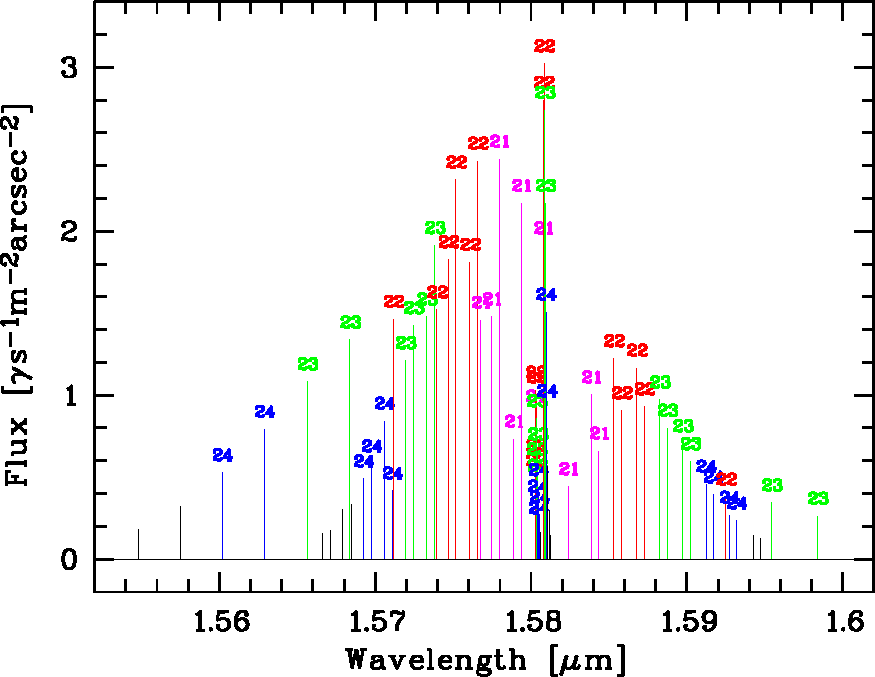
\includegraphics[width=10cm,clip=true]
{figures/scd_ploto2a01band.pdf}
\caption[]{B group identifications of the transitions of the band
O$_2$(a-X)(0-1) with a similar rotational upper state (cf.
Table~\ref{tab:Bgroups}). The tabulated wavelengths and zenithal mean fluxes of
the lines of the 9 different branches (3 R-, 3 Q-, and 3 P-branches) are shown
(cf. Figure~\ref{fig:ohband}).}
\label{fig:o2a01band}
\end{figure}

The wavelength range from the near-UV to the near-IR is characterised by strong
emission lines. Most of them constitute band structures. This airglow (see
Khomich et al.~\cite{KHO08} for a comprehensive discussion) mostly originates
in the mesopause region at about 90\,km. In addition, some lines arise in the
ionospheric F2-layer at about 270\,km. In general, airglow is caused by
chemiluminescence, \ie\ chemical reactions that lead to light emission by the
decay of excited electronic states of reaction products. Apart from atomic
oxygen and sodium, the oxygen (O$_2$) and hydroxyl (OH) molecules are the most
important reaction products in this context. In general, airglow lines show
strong variability from time scales in the order of minutes to years. This
behaviour can be explained by the solar activity cycle, seasonal changes in
temperature, pressure, and chemical composition of the emission layers, the
day-night contrast, dynamical effects such as gravity waves, or geomagnetic
disturbances.

The SKYCORR project aims at correcting airglow emission in science spectra by
means of reference sky spectra taken at a different time. As the airglow is
highly variable, the strength of the emission lines in a reference spectrum has
to be adapted, though. This is achieved by a fitting procedure that is
discussed in Section~\ref{sec:linefit}. Since emission lines belonging to the
science target should not be reproduced by the optimised sky spectrum and
finally removed, it is advisable to adapt as many lines as possible by a
single fitting parameter. Every group should contain airglow lines that are not
affected by object lines and that can be used to determine a realistic
correction factor for the reference sky spectrum. The number of lines that can
be combined is limited by the fact that they should show an almost identical
variability behaviour.

As basis for the definition of suitable line groups, the airglow line model
developed in the course of the SM-01 project for an advanced sky background
model for \ac{ESO} exposure time calculators was used (see \cite{SM01} User
Manual; Noll et al.~\cite{NOL12}). This semi-empirical model consists of a line
list with line intensities for mean observing conditions and prescriptions for
the correction of the line strength depending on molecular species, solar
activity, season, night time, and zenith distance of the target. The latter
three input parameters can be retrieved from the \ac{FITS} header of the sky
spectrum file. The solar activity is provided as solar radio flux at 10.7\,cm
either directly by {\sc solflux} in the parameter file or by the corresponding
monthly average (default) in a file offered by {\tt www.spaceweather.gc.ca}
(see Section~\ref{sec:params}). In the wavelength range from $0.3143$ to
$0.9228$\,\mum{}, the line list consists of data taken from Cosby et
al.~\cite{COS06} (supplemented by unpublished UVES 800U data) who incorporated
the UVES-based sky emission line atlas of Hanuschik \cite{HAN03}. At longer
wavelengths the calculated OH lines of Rousselot et al.~\cite{ROU00} were
included. However, their line strengths were corrected for the Einstein factors
of Goldman et al.~\cite{GOL98} instead of using the original, outdated ones of
Mies~\cite{MIE74}. This resulted in correction factors for OH band strengths
between 0.38 and 2.06. Moreover, the flux decrease of airglow lines by
molecular absorption in the lower atmosphere was corrected by the
multiplication of the airglow line spectrum with Doppler line widths for
typical temperatures of about 200\,K by the high-resolution
($\lambda / \Delta\lambda \approx 10^6$) Paranal annual-mean transmission
curve for an airmass of 1.25\footnote{Although the atmospheric
transmission depends on airmass and weather conditions, only a fixed airglow
flux correction was applied in order to avoid time-consuming calculations at
very high resolution and the input of temperature and water vapour profiles.
Moreover, the optical airglow atlas of Hanuschik \cite{HAN03} is also
characterised by a fixed transmission correction due to the use of UVES mean
spectra. For most observing conditions, the deviation of the true airglow
absorption from the assumed one is expected to be minor in terms of the results
of SKYCORR.} (see Noll et al. \cite{NOL12}). The transmission curve was
computed by means of the radiative transfer code LBLRTM (see Clough et al.
\cite{CLO05} and \cite{LBLRTM}). Note that SKYCORR applies the Paranal mean
transmission curve for zenith (corrected for the target airmass) to the
unextincted fluxes in the input line list. For this purpose, the line list
contains separate columns for unextincted line fluxes and zenithal transmission
values. Finally, the Rousselot et al.~lines were scaled to the Cosby et
al.~lines between $0.642$ and $0.858$\,\mum{}. The strongest O$_2$ bands in the
near-IR at $1.27$ and $1.58$\,\mum{} were included in the line list by adding
data from the HITRAN database (see Rothman et al.~\cite{ROT09} and
\cite{HITRAN}). The mean band strength was roughly estimated evaluating the
ratio of O$_2$ to OH lines in 26 IR X-Shooter spectra. For this purpose, the
O$_2$ lines had to be extincted depending on the airmass values of the
X-Shooter spectra. In the case of the $1.27$\,\mum{} band, this caused
significant changes in the line fluxes due to the strong resonant absorption of
airglow photons by tropospheric/stratospheric O$_2$ molecules in the ground
state.

The SM-01 sky model assigns the listed lines to five different variability
classes (see Figure~\ref{fig:varclasses}). These variability classes result
from analysing a sample of 1189 optical FORS spectra (Patat~\cite{PAT08}). From
this sample, the lines' dependence on solar radio flux and time of observation
(see Figure~\ref{fig:illfeatvar}) was derived. The latter was quantified using
a grid of six double month periods starting with Dec/Jan and three night time
bins of equal length. The reference line strengths in the line list represent
the mean of the five solar activity cycles 19 to 23, \ie\ the years 1954 to
2007.

Assigning airglow lines to the classes (1) green O\,I, (2) Na\,I\,D,
(3) red O\,I, (4) OH, and (5) O$_2$ using the rough predictions from the sky
model is not sufficient for achieving a line intensity accuracy on the percent
level and better, which is required for a sky subtraction procedure like
SKYCORR. Typically, intensity variations of lines within a variability class
are larger. The ratios of line strengths of different variability classes vary
by a factor of two or even more.

In principle, an identical variability behaviour can be expected for
transitions with the same upper energy level. In this case, the ratios of line
intensities should be fixed and only determined by quantities such as Einstein
coefficients and statistical weights. On the other hand, the excitation and
population of different energy levels depends on variable quantities such as
temperature, pressure, and chemical abundances. Therefore, it is a promising
ansatz to define line groups depending on the upper energy level. However,
taking all relevant energy levels of the molecules OH and O$_2$ into account
would result in a very large number of line groups. Moreover, each group would
consist of only a few significant lines. This would result in statistical
fluctuations, which could make the line intensity correction uncertain if
crucial lines of a group were affected by, \eg, CCD defects or object emission
lines (see Section~\ref{sec:linefit}). Fortunately, as their energies are
rather different, it is possible to separate electronic, vibrational, and
rotational transitions of molecules. The electronic/vibrational transition
determines the band and the rotational transition identifies a single line or
doublet (as in case of OH) within a band. Since the distribution of energy
levels is very similar for all bands of an electronic transition, each line can
be assigned to two different classes that are defined by the upper vibrational
and rotational state. This approach reduces the number of required line groups
significantly. Moreover, for OH only the electronic ground state is relevant,
which splits up into the sub-levels $X^2\Pi_{1/2}$ and $X^2\Pi_{3/2}$ due to the
coupling of spin and orbital angular momentum (see Rousselot et
al.~\cite{ROU00}). For O$_2$, the electronic transitions are more important
than the vibrational ones, since the intensity differences of the bands of an
electronic transition are very large. Consequently, there are only three O$_2$
bands that significantly contribute to the airglow, namely
O$_2$(b-X)(0-1)\footnote{The notation used is as follows: molecule (upper -
lower electronic state) (upper - lower vibrational state). The letters `a',
`b', and 'X' are shortcuts for the states  $a^1\Delta_g$, $b^1\Sigma^+_g$, and
$X^3\Sigma^-_g$. The vibrational states are numbered depending on the energy
and starting from 0 for the lowest level.} (the very strong (0-0) band is
almost completely absorbed in the lower atmosphere), O$_2$(a-X)(0-0), and
O$_2$(a-X)(0-1).

Tables~\ref{tab:Agroups} and \ref{tab:Bgroups} list the final grouping of
airglow lines. Line groups with the same upper electronic/vibrational level are
called ``A groups'' and those with the same (OH) or a similar (O$_2$) upper
rotational level are labelled as ``B groups''. Most OH bands (apart from a
few very weak ones) are identified in the Figures~\ref{fig:ohbands_opt} and
\ref{fig:ohbands_ir}. Although bands such as OH(4-1) and OH(4-2) have the same
upper vibrational level, they represent independent variability groups.
Although significantly increasing the number of A groups, the fact that real
data suffer from calibration uncertainties, makes this procedure a necessity.
As OH bands with the same upper vibrational level are widely separated, it is
therefore safer to vary such bands independently. Figures~\ref{fig:ohband},
\ref{fig:o2b01band}, \ref{fig:o2a00band}, and \ref{fig:o2a01band} show
identifications of the rotational B groups for an example OH band,
O$_2$(b-X)(0-1), O$_2$(a-X)(0-0), and O$_2$(a-X)(0-1), respectively. Although
the two O$_2$(a-X) bands belong to the same roto-vibrational system, their
B groups were defined separately due to the completely different line flux
distribution which is caused by self absorption in the (0-0) band. B groups of
O$_2$ bands consist of lines from two rotational upper levels in order to
make sure that enough lines can be identified for the group scaling (see
Section~\ref{sec:linefit}). The weak lines of each band are not included in a B
group as they are difficult to fit. Furthermore, this measure avoids a
degeneration of fit parameters.

The described grouping is reminiscent of the approach of Davies~\cite{DAV07}.
However, it is much more complex, since Davies only incorporates near-IR OH
bands, O$_2$(a-X)(0-0), and two rotational groups resembling our B\,2 and B\,4
classes (see Table~\ref{tab:Bgroups}).

%-------------------------------------------------------------------------------
\subsection{Airglow line fitter}\label{sec:linefit}
%-------------------------------------------------------------------------------
To prepare a reference sky line spectrum taken at a different time than the
corresponding science spectrum for a background subtraction, this reference
spectrum has to be adapted. To this end, Davies~\cite{DAV07} sub-divides the
wavelength range into sections depending on the OH band structure and
subsequently scales these sections independently according to the sections'
flux ratio of science and sky spectra. Problematic are cases where different
line groups have significant overlap. While the OH bands covered in SINFONI
$H$-band spectra exhibit only little overlap and no significant band of other
molecules are present, at lower wavelengths the situation is less favourable
(see Section~\ref{sec:airglow}). Even so, measuring the scaling factors for
groups with the same upper rotational level is difficult. Here, the flux of
individual lines has to be derived, which requires that the selected lines are
isolated. Typically, this is not the case for Q transitions, which are
characterised by a constant total angular momentum (see
Figure~\ref{fig:ohband}). Furthermore, the separation of variability groups
becomes even more difficult if the spectral resolution is relatively low as in
the case of the FORS spectra shown in Figure~\ref{fig:varclasses}.

To overcome these limitations, the SKYCORR project pursues a completely
different approach to obtaining the scaling factors for the different line
groups defined in Section~\ref{sec:airglow}. In SKYCORR, the contributions of
the line groups to each pixel of the sky spectrum are estimated. Subsequently,
the resulting spectra for each line class ($\le 100$\% of the total sky flux)
are scaled.

This is performed applying the airglow model presented in the previous section.
The wavelengths and intensities of the lines and their group identifications
can be converted into intensities of the different line groups for each pixel.
This requires a convolution of the lines from the line list with a kernel
similar to the instrumental profile of the observed spectra. The mean FWHM of
the sky lines, which was obtained in a previous step (see
Section~\ref{sec:FWHM}), is used for creating a sufficently realistic Gaussian
kernel. In order to treat intensity ratios of overlapping lines as
realistically as possible, the airglow variability model from Noll et
al.~\cite{NOL12} (see Section~\ref{sec:airglow}) was included. This allows one
to rougly correct for the influence of solar activity, season, and night time
on the main line variability classes green O\,I, Na\,I\,D, red O\,I, OH, and
O$_2$.

Different line groups contributing to the same pixel implies that the sky
scaling factors cannot be derived by a simple division of line fluxes of
science and sky spectrum anymore. Instead, each scaling factor of the
individual line groups has to be included in a fitting procedure as a free
fitting parameter. For this purpose, the C library MPFIT by
C.~Markwardt~\cite{CMPFIT} (see Section~\ref{sec:FWHM}) was used. The $\chi^2$
minimisation procedure of this routine is based on a Levenberg-Marquardt
technique (see Mor\'e et al. \cite{MOR80}), an iterative search algorithm
characterised by gradient-controlled jumps in parameter space. Since this
technique is potentially prone to finding local minima, reasonable starting
values and constraints for the fit parameters are required. For this reason,
the mean ratios of the line peaks in the science and sky spectrum are
calculated for each line group (see Section~\ref{sec:airglow}). Only those
spectrum pixels are included that were identified as line peak (see
Section~\ref{sec:linesearch}) or are separated from a peak by not more than
half a line FWHM (see Section~\ref{sec:FWHM}) and have a relative contribution
of the selected line group of at least {\sc weightlim} (default: 0.67; see
Section~\ref{sec:params}). Moreover, pixels with unreasonable flux ratios are
rejected by applying a global $\sigma$ limit that is derived from the full
set of line peaks and is provided by the parameter {\sc siglim} (default: 15;
see Section~\ref{sec:params}). In this way, strong object emission lines can be
identified in the science line spectrum and excluded. Finally, the
$\sigma$-clipping approach with variable $\sigma$ limit described in
Section~\ref{sec:FWHM} is applied to the selected pixels of each group
separately in order to further improve the pixel selection. The remaining
pixels of this procedure are taken for the initial line group scaling {\em and}
fitting algorithm, \ie\ only those pixels are considered for the $\chi^2$
calculation. If suitable pixels cannot be found for a line group, a mean
flux ratio of the corresponding system of electronic transitions (\eg\ OH; see
Section~\ref{sec:airglow}) or a global flux ratio is taken for A groups and a
value of 1 is assumed for B groups. For most sky spectra this approach should
result in a good first guess sufficient for achieving rapid convergence to the
global minimum (see Section~\ref{sec:evaluation}).

As an option the fitting can be restricted to uncertain line groups only. The
decision on the group selection depends on the parameter {\sc fitlim} (see
Section~\ref{sec:params}) which provides a limiting ratio of the RMS and
the mean of the group-specific scaling factors. By default this value is set
to 0, \ie\ all fittable line groups are considered.

%-------------------------------------------------------------------------------
\subsection{Correction of wavelength grid}\label{sec:wavegrid}
%-------------------------------------------------------------------------------

Since the sky lines of the science spectrum are removed by a scaled reference
sky line spectrum, it is imperative that the wavelength grids of both spectra
are aligned. Differences of less than a pixel can already significantly
deteriorate the quality of the sky subtraction. Relatively large deviations can
occur if a lamp spectrum taken in daytime at different ambient conditions than
the science spectrum is used for the wavelength calibration. However, even
subpixel shifts that are routinely observed in data taken under perfect
conditions can cause problems.

For this reason, SKYCORR offers optional correction of the wavelength grid by
applying a Chebyshev polynomial of degree
$n_\mathrm{w}$
\begin{equation}
\lambda' = \sum_{i = 0}^{n_\mathrm{w}} c_i t_i,
\end{equation}
where
\begin{equation}
t_i = \left\{ \begin{array}{ll}
1 & \textrm{for\ } i = 0 \\
\lambda & \textrm{for\ } i = 1 \\
2 \, \lambda \, t_{i-1} - t_{i-2} & \textrm{for\ } i \ge 2
\end{array} \right.
\end{equation}
and $\lambda$ ranging from -1 to 1. The temporary conversion of the wavelength
grid to a fixed interval results in coefficients $c_i$ independent of the
wavelength range and step size of the input spectrum. The wavelength solution
is not changed if $c_1 = 1$ and $c_i = 0$ for all other $i$. It is possible
to set an individual start value for the constant term $c_0$ via the parameter
{\sc cheby\_const} (see Section~\ref{sec:params}). In this way, significant
possible shifts between the wavelength grids of the science and the sky
spectrum can be considered.

The coefficients $c_i$ are determined by an iterative procedure. This process
is initialised with two subsequent estimates (for a better $\sigma$-clipping)
and a fit of the line flux correction factors (see Section~\ref{sec:linefit}).
During this first iteration the wavelength grid remains untouched. In the next
step, the coefficients $c_0$ and $c_1$ are fitted using MPFIT. Now, a new
estimate is calculated and the line flux correction factors are fitted again.
Then the next iteration starts by fitting the wavelength grid, now applying a
Chebyshev polynomial of degree 2. After that, the line scaling factors are
adapted again in order to incorporate the change of the wavelength grid. Each
iteration increases $n_\mathrm{w}$ by 1 and uses the results of the
previous iteration as input. The search for the best polynomial degree is
controlled by the three input parameters {\sc cheby\_min}, {\sc cheby\_max},
and {\sc wtol} (see Section~\ref{sec:params}). The iteration process is stopped
once the maximum polynomial degree given by {\sc cheby\_max} is reached. For a
value of -1, no wavelength grid correction is performed. The parameter
{\sc cheby\_min} indicates the minimum degree, \ie\ the minimum number of
iterations. For $n_\mathrm{w}$ not less than {\sc cheby\_min}, the code checks
whether the resulting $\chi^2$ shows a relative $\chi^2$ improvement of at
least {\sc wtol} (default: $1 \times 10^{-3}$) compared to the best $\chi^2$, so
far. If this is not the case the procedure stops and the results for the
polynomial with the lowest $\chi^2$ are taken. An exception is a choice of
{\sc cheby\_min}~>~{\sc cheby\_max}. In this case, the code runs until
{\sc cheby\_max} is reached and the corresponding results for this degree are
taken, regardless of the results for the lower polynomial degrees. The default
values for {\sc cheby\_max} and {\sc cheby\_min} are 7 and 3, respectively.

Independent of the use of a Chebyshev polynomial, the modified sky spectrum has
to be rebinned to the wavelength grid of the science spectrum. For this task,
the code offers two options, which can be selected by the parameter
{\sc rebintype} (see Section~\ref{sec:params}). The first method adds up the
fractional fluxes of input pixels contributing to the wavelength range of the
output pixel. The second approach is based on the convolution of the input
spectrum with a pixel-dependent asymmetric damped sinc kernel
\begin{equation}
f(k) = e^{-((k - s) / \delta)^2} \, \frac{\sin(\pi (k - s))}{\pi (k - s)},
\end{equation}
with $k$ being an integer variable ranging from $-k_\mathrm{max}$ to
$k_\mathrm{max}$. The damping constant $\delta$ and the kernel radius
$k_\mathrm{max}$ are fixed and have the values 3.25 and 5. The parameter $s$ is
the subpixel shift of the sky spectrum relative to the science spectrum. It is
a function of the pixel position and ranges from $-0.5$ to $0.5$. For shifts
above half a pixel, complete pixels are treated by a simple renumbering of the
input pixels in the output spectrum. No convolution is performed for this
integer part of the pixel shift. The approach is similar to the one used in the
IDL routine ``sshift2d.pro'' of the Lowell Buie Library \cite{SINC}. However,
the original programme is for a constant shift of the entire spectrum only. A
wavelength-dependent shift is not a problem as long as the amount of the shift
changes slowly with the spectrum pixels and the pixel size is nearly constant
for the whole input and output wavelength grids. These requirements are
sufficiently met if inconsistencies of the wavelength grids are in the order of
1\,pixel and if the functional dependence of differences can be described by a
low order polynomial. The relatively complicate rebinning method described
above is able to effectively suppress broadening of spectral lines, which
typically occurs if a spectrum is rebinned to a shifted grid of similar pixel
size. The line-broadening suppression is achieved by alternating positive and
negative contributions to the kernel as incorporated in the sinc shift method.
Therefore, the sinc shift method produces the best results if significant
subpixel shifts close to half a pixel are frequent. However, for a very good
agreement of the wavelength grids with subpixel shifts close to zero, it might
be better to use the simple rebinning method. In such a case, the relatively
broad sinc kernel influences the spectrum more than simple regridding.
